\documentclass[man,12pt,floatsintext, a4paper]{apa6}\usepackage[]{graphicx}\usepackage[]{color}
%% maxwidth is the original width if it is less than linewidth
%% otherwise use linewidth (to make sure the graphics do not exceed the margin)
\makeatletter
\def\maxwidth{ %
  \ifdim\Gin@nat@width>\linewidth
    \linewidth
  \else
    \Gin@nat@width
  \fi
}
\makeatother

\definecolor{fgcolor}{rgb}{0.345, 0.345, 0.345}
\newcommand{\hlnum}[1]{\textcolor[rgb]{0.686,0.059,0.569}{#1}}%
\newcommand{\hlstr}[1]{\textcolor[rgb]{0.192,0.494,0.8}{#1}}%
\newcommand{\hlcom}[1]{\textcolor[rgb]{0.678,0.584,0.686}{\textit{#1}}}%
\newcommand{\hlopt}[1]{\textcolor[rgb]{0,0,0}{#1}}%
\newcommand{\hlstd}[1]{\textcolor[rgb]{0.345,0.345,0.345}{#1}}%
\newcommand{\hlkwa}[1]{\textcolor[rgb]{0.161,0.373,0.58}{\textbf{#1}}}%
\newcommand{\hlkwb}[1]{\textcolor[rgb]{0.69,0.353,0.396}{#1}}%
\newcommand{\hlkwc}[1]{\textcolor[rgb]{0.333,0.667,0.333}{#1}}%
\newcommand{\hlkwd}[1]{\textcolor[rgb]{0.737,0.353,0.396}{\textbf{#1}}}%
\let\hlipl\hlkwb

\usepackage{framed}
\makeatletter
\newenvironment{kframe}{%
 \def\at@end@of@kframe{}%
 \ifinner\ifhmode%
  \def\at@end@of@kframe{\end{minipage}}%
  \begin{minipage}{\columnwidth}%
 \fi\fi%
 \def\FrameCommand##1{\hskip\@totalleftmargin \hskip-\fboxsep
 \colorbox{shadecolor}{##1}\hskip-\fboxsep
     % There is no \\@totalrightmargin, so:
     \hskip-\linewidth \hskip-\@totalleftmargin \hskip\columnwidth}%
 \MakeFramed {\advance\hsize-\width
   \@totalleftmargin\z@ \linewidth\hsize
   \@setminipage}}%
 {\par\unskip\endMakeFramed%
 \at@end@of@kframe}
\makeatother

\definecolor{shadecolor}{rgb}{.97, .97, .97}
\definecolor{messagecolor}{rgb}{0, 0, 0}
\definecolor{warningcolor}{rgb}{1, 0, 1}
\definecolor{errorcolor}{rgb}{1, 0, 0}
\newenvironment{knitrout}{}{} % an empty environment to be redefined in TeX

\usepackage{alltt}
\usepackage[latin1]{inputenc}
\usepackage{amsmath}
\usepackage{amsfonts}
\usepackage{amssymb}
\usepackage[american]{babel}
\usepackage{csquotes}
\usepackage[style=apa, sortcites=true,url=false, firstinits=true,doi=true,sorting=nyt, backend=biber]{biblatex}
\DeclareLanguageMapping{american}{american-apa}
\usepackage{geometry}
\usepackage{rotating}
\usepackage{graphicx}
\usepackage{units}
\usepackage{multicol}
\usepackage{multirow}
\usepackage{pdflscape}
\usepackage{subcaption}
\usepackage{xfrac}
\usepackage{color}
\usepackage{tikz}
\usepackage{xspace}
\usepackage{verbatim}
\usepackage[textfont=normalfont]{caption}
\usetikzlibrary{arrows,decorations.markings} 
\usetikzlibrary{arrows.meta}
\definecolor{lavendermagenta}{rgb}{0.93, 0.51, 0.93}

%version 2 started 14/9/2018
%updates made as indicated in commentsOSID.txt
%version 2 compiled and copy to GlautierBrudan2018OSIDRevised.pdf ci work/osid 2286
%from osid run vim -S osidbf.vim
%version 1 submitted to JEPLMC and OSF 19/1/2018
%work/osid c2012 19/1/2018
%rwork/e168 c2007 15/1/2018
%rwork/e175 c1830 1/9/2017
%see files osPages.pdf, experiments.pdf, osid.r (constructed from E168/E168a.r, E168/explore.r, E175/e175.r) run vim from rwork vim -S osid.vim
%final osidbf.vim
%files for export
%osid/ 		osid#2.Rnw
%			osidDisc.Rnw
%			osidIntro.Rnw
%			osidbf.Rdata
%			osidBFExport.r
%e168/		osid2Export.r
%			allData168a.Rdata		
%			allData168b.Rdata
%e175/		part1.Rdata
%			part2.Rdata
%functions/ generic.r
%compile and copy to GlautierBrudan2018OSID.pdf for OSF
%move tables compile to osidjeplmc19-01-18.pdf for sending to jeplmc commit 2012 along with coverletterJEPLMC.txt
\def\pc{/admin/}
%set to spg or admin
\newif\ifsurface
\surfacefalse
%\surfacetrue
%the root r-directory, where common directories and files stored e.g. rwork/functions, rwork/classes
%the data and r-code for the current document will be stored in e.g. rwork/current so functions could be accessed ../functions
\def\rroot{c:/users\pc documents/rwork/}
%define the latex root directory where bibliography stored and where latex /work directory exists
\def\lroot{c:/users\pc documents/latex/}
%pegs stuff needed in some documents
\ifsurface
 \def\proot{D:/Google Drive/PEGS/document/}
 \def\groot{d:/google drive/}
\else
 \def\proot{C:/Users\pc Google Drive/PEGS/document/}
 \def\groot{c:/users\pc google drive/}
\fi

%bibliography
\def\bd{c:/users\pc documents/latex/allbib.bib}
\addbibresource{\bd}

\AtEveryBibitem{% Clean up the bibtex rather than editing it see http://codydunne.blogspot.co.uk/2012/01/suppressing-bibtex-fields-for-specific.html
 \clearfield{note}
 \clearfield{number}
 \clearfield{month}
 \clearfield{eprint}
} 

\newcommand{\trw}{the Rescorla-Wagner model\xspace}
\newcommand{\Trw}{The Rescorla-Wagner model\xspace}
\newcommand{\trrw}{the reduced Rescorla-Wagner model\xspace}
\newcommand{\Trrw}{The reduced Rescorla-Wagner model\xspace}
\newcommand{\tpcm}{the Pearce configural model\xspace}
\newcommand{\Tpcm}{The Pearce configural model\xspace}
\newcommand{\rw}{Rescorla-Wagner\xspace}
\newcommand{\rwm}{Rescorla-Wagner model\xspace}
\newcommand{\cm}{configural model\xspace}
\newcommand{\tcm}{the configural model\xspace}
\newcommand{\Tcm}{The configural model\xspace}
\newcommand{\trhs}{the right-hand side\xspace}
\newcommand{\tlhs}{the left-hand side\xspace}
\newcommand{\rhs}{right-hand side\xspace}
\newcommand{\lhs}{left-hand side\xspace}
\newcommand{\ssr}{smaller-sooner reward\xspace}
\newcommand{\llr}{larger-later reward\xspace}
\newcommand{\dd}{delay-discounting\xspace}
\newcommand{\prz}{preference-reversal-zone\xspace}
\newcommand{\me}{MECA\xspace}
\newcommand{\mem}{MECA model\xspace}
\newcommand{\tme}{the MECA model\xspace}
\newcommand{\Tme}{The MECA model\xspace}
\newcommand{\trme}{the reduced MECA model\xspace}
\newcommand{\Trme}{The reduced MECA model\xspace}
\newcommand{\lli}{log-likelihood\xspace} %suffix i to disambiguate
\newcommand{\llis}{log-likelihoods\xspace}
\newcommand{\ml}{maximum likelihood\xspace}
\newcommand{\Ml}{Maximum likelihood\xspace}
\newcommand{\Cc}{Classical conditioning\xspace}
\newcommand{\cc}{classical conditioning\xspace}
\newcommand{\Pc}{Pavlovian conditioning\xspace}
\newcommand{\cs}{conditioned stimulus\xspace}
\newcommand{\css}{conditioned stimuli\xspace}
\newcommand{\Css}{Conditioned stimuli\xspace}
\newcommand{\us}{unconditioned stimulus\xspace}
\newcommand{\uss}{unconditioned stimuli\xspace}
\newcommand{\Uss}{Unconditioned stimuli\xspace}
\newcommand{\ur}{unconditioned response\xspace}
\newcommand{\urs}{unconditioned responses\xspace}
\newcommand{\Urs}{Unconditioned responses\xspace}
\newcommand{\cri}{conditioned response\xspace} %suffix i to disambiguate
\newcommand{\cris}{conditioned responses\xspace} 
\newcommand{\Cris}{Conditioned responses\xspace}
\newcommand{\mcet}{multiple-context cue-exposure therapy\xspace}
\newcommand{\Mcet}{Multiple-context cue-exposure therapy\xspace}
\newcommand{\mcets}{multiple-context cue-exposure therapies\xspace}
\newcommand{\Mcets}{Multiple-context cue-exposure therapies\xspace}
\newcommand{\cet}{cue-exposure therapy\xspace}
\newcommand{\Cet}{Cue-exposure therapy\xspace}
\newcommand{\cets}{cue-exposure therapies\xspace}
\newcommand{\Cets}{Cue-exposure therapies\xspace}
\usepackage{color}
\usepackage{soul}
\newcommand{\hlc}[2][yellow]{ {\sethlcolor{#1} \hl{#2}} }
\definecolor{bkgdcol}{rgb}{0.86,0.86,0.86}
\definecolor{lavendermagenta}{rgb}{0.93, 0.51, 0.93}


\graphicspath{{../../../../workspace/simlib/}}

\author{Steven Glautier and Ovidiu Brudan}

\affiliation{Southampton University}

\title{Stable Individual Differences in Occasion Setting}
\shorttitle{Differences in Occasion Setting}
\note{6506 words 12/10/18}
\authornote{Correspondence should be addressed to Steven Glautier, School of Psychology, University of Southampton, Southampton, SO17 1BJ, United Kingdom. E-mail: spg@soton.ac.uk, Tel: (+44) 023 8059 2589. Acknowledgements to student volunteer research assistant Jessica Richards for help with data collection.}

\abstract{In the current investigation we classified participants as inhibitors or non-inhibitors depending on the extent to which they showed conditioned inhibition in a context that had been used for extinction of a conditioned response. This classification enabled us to predict participant responses in a second experiment which used a different design and a different experimental task. In the second experiment a feature-negative discrimination survived reversal training of the feature to a greater extent in the non-inhibitors than in the inhibitors and this result was supported by Bayesian analyses. We propose that the fundamental distinction between inhibitors and non-inhibitors is based on a tendency to utilise first-order (direct associations) or second-order (occasion-setting) strategies when faced with ambiguous information and that this classification is a stable individual differences attribute. (138 words)}

\keywords{associative learning, inhibition, occasion-setting, response-recovery, feature-negative discrimination, reversal, individual differences}

\leftheader{Glautier, Brudan}
\IfFileExists{upquote.sty}{\usepackage{upquote}}{}
\begin{document}
\maketitle


\setlength{\parindent}{1cm}
\section{Introduction}
Associative learning plays a crucial role in the survival of organisms by facilitating the acquisition of responses to stimuli which signal significant events. However, acquisition is only half of the story because in an ever-changing environment a response that was once appropriate may become redundant or even maladaptive if it continues to occur when the environmental conditions change. For example an animal may learn that a particular location is a good source of food but if it continues returning to that location after the source is exhausted it will waste energy that could be better spent foraging elsewhere. Extinction is one process by which an organism may adapt to changes in environmental conditions. Procedurally, extinction involves presenting a \cs (CS) alone, without the \us (US) it was previously paired with. During extinction the \cri (CR) produced by the CS is observed to decline in magnitude and probability until at some point extinction appears to be complete. Superficially extinction resembles unlearning and in one of the most widely cited theoretical models of associative learning, \trw \parencite{RescorlaWagner1972}, extinction is exactly that -- the undoing, without leaving a trace, of a previously learned association.

However, it is well established that extinction cannot be understood as simple unlearning. Spontaneous recovery and renewal are among those phenomena which demonstrate that traces of the original learning survive extinction \parencite[e.g.][]{Bouton1994}. Spontaneous recovery refers to renewed CRs that occur when the CS is presented after a delay following extinction. \citeauthor{Brooks1993} trained rats with a tone CS signalling delivery of food then presented the CS alone during an extinction phase. Responding clearly declined during extinction. Animals were then given test presentations of the CS either five hours or six days after extinction. Animals tested five hours after extinction showed a slight increase in responding to the CS compared to that seen at the end of extinction. In contrast, animals tested six days after extinction showed dramatically increased responding to the CS compared to that seen at the end of extinction. In fact responding in the test was slightly higher than it was before extinction, a clear spontaneous recovery effect showing that extinction did not simply erase what had been learned during acquisition \parencite{Brooks1993}. Renewal refers to renewed CRs consequent to a contextual change after extinction. \let\old\postnotedelim \renewcommand{\postnotedelim}{ }\citeauthor[][(Experiment 1)]{BoutonKing1983} \renewcommand{\postnotedelim}{\old} trained rats with a tone CS signalling electric shock in one context, context $A:$ ($A:T+$ trials\footnote{The colon indicates that identifier A refers to a contextual cue. In contrast an undecorated identifier (e.g. $T$) refers to a discrete cue. When an experiment only involves a single US the  `+' sign indicates a trial with the US and a `-' sign indicates a trial without the US.}), and then extinguished the CS in another context, context $B:$ ($B:T-$ trials), before testing the CS back in context $A:$. Clear extinction effects were seen but responding returned when the CS was tested in context $A:$. These results were supported by further tests which showed that the renewal effect was not mediated by the excitatory properties of context $A:$ \parencite{BoutonKing1983}. Other rat studies, where testing was carried out in a novel context $C:$ (an ABC design as opposed to an ABA design), confirmed that renewal effects do not depend on the excitatory properties of the test context \parencite{BoutonBolles1979}.

Results such as these present important problems for learning theories and in what follows we describe two leading explanations for renewal to set the stage for the experiments to be presented below. The central question is, how we can understand the decline in responding that is seen during extinction when there is clear evidence that the original learning remains intact? We argue that two leading explanations for renewal, one based on context inhibition and one based on occasion-setting, are not mutually exclusive \parencite[e.g.][]{BoutonNelson1994}. The experiments reported below show that human participants may be categorised into one of two groups. In one group, inhibitors, renewal seems to be controlled by inhibitory associations involving the experimental context. In another group, non-inhibitors, we argue that renewal is controlled by an occasion-setting mechanism. The classification of participants into these two groups appears to be relatively stable, allowing predictions to be made across different experimental procedures, and indicates some practical implications. We leave consideration of these practical implications for the Discussion to focus here on two theoretical explanations for renewal.

In associative models learning is conceptualised as changes in the strength of associative links between mental representations of CSs and USs. We review here the operation of \trw as a `standard' model of associative learning \parencite{RescorlaWagner1972}. Although \trw was developed as a model of \Pc in animals its principles are sufficiently general to have been successfully imported into new domains. \Trw has been considered a viable candidate model in a variety of human learning tasks including predictive, causal, and Pavlovian learning \parencite[e.g.][]{DickinsonShanksEtAl1984,Lachnit1988,ChapmanRobbins1990}. In \trw, in the case of simple excitatory learning, where a CS is repeatedly paired with a US, the association strength, $V$, increases towards an asymptote and is greater than zero. When $V>0$ the CS is said to be excitatory and presentation of the CS activates the US representation -- informally presentation of the CS leads to an expectation of the US through spreading activation. $V$ can also be reduced when an expected US fails to occur, for example during extinction, and this may result in $V$ becoming negative in which case the CS is said to be an inhibitor. When there is an inhibitory CS-US association presentation of the CS effectively suppresses expectation of the US. \Trw formally explains renewal effects though a mechanism known as `protection-from-extinction' in which the extinction context develops inhibitory associative strength as detailed in the following paragraph.

\begin{equation} 
\label{eq:rwSimple} \Delta V=\alpha \beta (\lambda-\Sigma V)
\end{equation}

Equation \ref{eq:rwSimple} is the fundamental \rwm learning equation\label{lab:extstr}. In Equation
\ref{eq:rwSimple} $\Delta V$ is the change in the associative strength between the mental
representation of a predictive stimulus (such as a tone CS) and the representation of the outcome
(such as a shock US) that occurs on a single learning trial. $\Delta V$ is a function of two
learning rate parameters, $\alpha$ for the CS and $\beta$ for the US, and the parenthesised error
term. In the error term $\lambda$ is the value of the US on that trial (usually modelled as 1 or 0 for the
occurrence and non-occurrence of the US, respectively) and $\Sigma V$ is the summed associative
strength of all the predictors that are present on the trial. To see how inhibitory learning takes
place during extinction consider the associative strength of cue $A$ after an acquisition phase
involving a series of $A\!:\!A+$ trials. Asymptotically $V_{A:}+V_A \rightarrow 1$ and
$\sfrac{V_{A:}}{V_A}=\sfrac{\alpha_{A:}}{\alpha_A}$. Following acquisition there is an extinction
phase involving $\!B:\!A-$ trials. At the start of extinction $V_{B:}=0$ and $\Sigma V=V_{B:}+V_A>0$.
During extinction $\lambda=0$ and since $\alpha>0$ and $\beta>0$ then $\Delta V <0$. Since
$V_{B:}=0$ at the start of extinction $V_{B:}$ becomes negative during extinction and $V_A$
declines. Learning (and responding) during extinction stops when $V_{B:}+V_A=0$ and at this point $B\!:$
is inhibitory ($V_{B:}<0$) while $A$ remains excitatory ($V_A>0$). The presence of inhibitory $B\!:$ is
said to protect $A$ from extinction.

Protection from extinction effects have been demonstrated by presenting a discrete inhibitory CS in compound with a CS during extinction \parencite[e.g.][]{Rescorla2003}. However, there are few experiments which have found evidence for the context developing inhibition during extinction, as would be expected following the theoretical analysis above, calling into question the proposal that protection from extinction could explain the renewal effects that we are considering. For example, in the study mentioned above \citeauthor{BoutonKing1983} used a summation test to look for context inhibition \parencite{BoutonKing1983}. A summation test involves presenting an excitatory cue in compound with a putative inhibitor \parencite{Rescorla1969} and in this case \citeauthor{BoutonKing1983} presented an excitatory CS in the extinction context but no inhibition was detected. More recently \textcite{PolackLabordaEtAl2012} reported evidence for extinction contexts becoming inhibitory in a summation test, and also in a retardation test in which learning is acquired more slowly in the presence of the inhibitor than in its absence \parencite{Rescorla1969}. \citeauthor{PolackLabordaEtAl2012} found clearest evidence for context inhibition during extinction when using short inter-trial-intervals and suggest that this variable may explain why there are few reports of context inhibition in the literature. Again using a summation test but this time using human subjects both \textcite{NelsonSanjuanEtAl2011} and \textcite{HavermansKeukerEtAl2005} found reduced conditioned suppression when an excitatory cue was presented in the extinction context indicating that the context was inhibitory. However, these results are ambiguous since \textcite{NelsonSanjuanEtAl2011} demonstrated that conditioned suppression was also reduced when the excitatory cue was presented in an associatively neutral context. Thus, any putative conditioned inhibitory effect of the extinction context added nothing to conditioned suppression produced by a novel cue-context combination. However, \textcite{Glautier2013a} found clear evidence for context inhibition with appropriate controls using a predictive learning task (see Discussion, page \pageref{lab:previousCI}) so it seems as though it may be premature to rule-out a role for protection from extinction in extinction and renewal effects.

Partly as a result of failures to confirm that extinction contexts become conditioned inhibitors alternatives to the protection from extinction explanation for renewal have been developed. Occasion setters are stimuli that can be shown to influence the expression of an association between a CS and a US without themselves being directly associated with the US. Instead they function by controlling an `and-gate' which switches the CS-US association on or off \parencite{Bouton1994,Holland1992,Swartzentruber1995}. An occasion-setting mechanism is illustrated in Figure \ref{fig:extinctionStructures} where it is contrasted with \trw. Figure \ref{fig:extinctionStructures} shows the hypothesised associative structures that are formed after acquisition (left-hand side) and after extinction (right-hand side). $CS_A$ was paired with the US during an acquisition phase to produce an $A\rightarrow US$ association (left) and then, in a new context, context $B:$,  $CS_A$ was extinguished by presentation without the US. According to \trw, as explained above, this produces an inhibitory association between context $B:$ and the $US$ (bottom right). In contrast, in an occasion-setting model, it is assumed that context $B:$ forms an inhibitory link with the $A\rightarrow US$ structure (top-right) so that when context $B:$ is present the association is switched off and switched on otherwise. We term direct associations between CSs and the US `first-order' and associations which operate on first-order associations `second-order'. It should be apparent that renewal of responding is predicted for the second-order model, as well as the first-order model, because when $CS_A$ is presented outside of context $B:$ the $A\rightarrow US$ association will be active.\label{lab:extstr1}

The current investigation follows-up the work of \textcite{Glautier2013a}. It was based on an analysis of renewal in which it was assumed that the two mechanisms outlined above could operate. During an extinction phase of a renewal experiment we assumed that participants could suppress responding by conditionalising an $A\rightarrow US$ association that had been learned during the acquisition phase on the experimental context or by learning that the context was inhibitory as illustrated in Figure \ref{fig:extinctionStructures}. In \citeauthor{Glautier2013a}, although there was a clear overall context inhibition effect, approximately 50\% of participants showed some responding to a test cue when it was presented in the extinction context. It was hypothesised that extinction in participants who failed to suppress responding in the extinction context summation test would have had extinction performance controlled by second-order associations. This is because one of the defining features of an occasion-setter is that its occasion-setting function is specific to a particular CS-US relation \parencite[e.g.][]{Holland1989,Holland1992}. Thus, if $B\!:$ has occasion set the $CS_A\rightarrow US$ relation then it should not affect another CS-US relation (e.g. $CS_D\rightarrow US$). In contrast, conditioned inhibition shows no such specificity since it operates on the US representation. Thus, if $B\!:$ has become inhibitory it should suppress responding to any excitatory cue it is compounded with. 

Of course a classification of participants based on a single test has little value unless there is some independent predictive value of that classification. Therefore we report below on two sequentially conducted experiments. Experiment 1 was a renewal experiment, based closely on \textcite{Glautier2013a}, which provided an inhibition score for each participant. On the basis of these scores participants were classified as inhibitors or non-inhibitors. Then,
in Experiment 2, participants underwent feature negative training\label{lab:extstr2}, followed by reinforcement of the feature, and then a test to see if the feature negative discrimination was disrupted. Feature-negative training is a procedure in which a cue is reinforced when it is presented alone and non-reinforced whenever it occurs in the presence of another cue (the feature negative). It was predicted that the feature negative discrimination would be maximally disrupted in the inhibitors, i.e. those predisposed to learn first order solutions. This would be consistent with previous reports which have shown that feature negative discriminations in which the feature is trained as an occasion-setter using serial presentation can be maintained after reinforced trials with the feature \parencite[e.g.][]{Holland1984, Rescorla1987, Holland1992}. The rationalisation of this prediction is illustrated in Figure \ref{fig:reversalStructures}\label{lab:reversalStructures}. After training with $A+$ and $AB-$ trials responding could be controlled by first-order associative structures (left-hand side, bottom) or by second-order structures (left-hand side, top). Following reinforcement of feature $B$ the second-order associative structures formed by the non-inhibitors will have an excitatory input to the US representation from $B$ (right-hand side, top). There is also an excitatory input to the US representation from $A$, but this association is gated closed by the presence of $B$. In contrast the inhibitors will have excitatory inputs to the US representation from both $A$ and $B$ (right-hand side, bottom). Consequently we predicted stronger responses in the $AB$ compound test for the inhibitors than for the non-inhibitors. 



\section{Experiment 1}
Participants took part in a computer-based predictive learning task during which they viewed a series of on-screen trials and were told that their task was to learn to predict the outcome of each trial on the basis of visual cues presented at the start of each trial. The trial outcomes were coloured flashes on the computer screen and the cues were visually distinctive objects which `fell' on each trial from the top to the bottom of the computer screen. Towards the end of the trial, which lasted about 5s in total, the objects passed a `sensor' located in the bottom part of the screen and the coloured flashes, when they occurred, were timed with and said to be triggered by the object passing the sensor. On each trial participants had to press a key to indicate their expectation, with respect to the outcomes, before the objects passed the sensor. There were three response options available; key-R to predicted a red flash, key-G to predict a green flash, or no-key to predict no flash. Participants were instructed to make as many correct predictions as possible but minimise incorrect predictions. Further details of the task are given in \textcite{Glautier2013a} and an illustrative video can be found at \url{https://tinyurl.com/y6v5unpj}. 

\subsection{Method}
Procedures were approved by the University of Southampton Research Governance Office and the School of Psychology's Ethics Committee.

\subsubsection{Participants}
Eighty participants took part. They were recruited by word of mouth and posted advertisement. Their mean age was 20.7 years (range 16-39) and they included 24 males. Participants were recruited in two distinct samples. The first sample of 28 was recruited, and tested, by JR from a local community in Wiltshire, UK. The second sample of 52 was recruited, and tested, by OB from the University of Southampton Highfield campus. Participants in the first sample were tested in various convenient community environments and paid �4 for their participation whilst participants in the second sample were tested in psychology research laboratories and given course credit for participation.

\subsubsection{Apparatus}
For the first sample the experiment was run on a laptop computer with a screen measuring 30.5 cm x 19.2 cm (W x H) running at 60hz. For the second sample the experiment was run on personal computers with screens measuring 41 cm x 26 cm (W x H) running at 75hz. In both cases the displays used 32 bit colour mode and pixel resolutions of 1440 x 900 and were controlled by computer programs written by the first author in Microsoft C\# language using Microsoft XNA Game Studio Version 3.1 for rendering of the experimental scenario.

\subsubsection{Design and procedure}
\label{sec:E1DandP}
Participants received a brief verbal introduction to the procedures and then signed a consent form before reading a more detailed on-screen description of the task. This description is provided in full as part of the illustrative video. Participants then had the opportunity to ask questions before the experimental procedure began. Table \ref{tab:designP1} shows the design for Experiment 1. The experiment contained acquisition, extinction, summation test, and recovery test phases. The table shows the trial types that were presented in each phase. Different phases took place in different contexts wherein the screen background changed. Acquisition, extinction, and the recovery test took place the three different contexts i.e. it was an ABC design. The screen backgrounds that served the roles of contexts $A:$, $B:$, and $C:$ were selected randomly without replacement from four possibilities for each participant. Context $B:$ was used for the summation test. The cue objects presented on each trial, serving the roles of $A$, $B$, $C$, and $D$, were selected randomly without replacement from 16 possibilities for each participant. The coloured flashes serving the roles of $X$ and $Y$ were selected randomly without replacement from two possibilities (red and green) for each participant. Outcome $Z$ designates the no-flash outcome. The phases were divided into blocks with each block containing equal numbers of each trial type. Trial order was randomised independently for each participant within block so there could be no more than four repeats of a trial type in a single sequence. Responses made in the summation test were used to classify participants as either non-inhibitors or inhibitors. After completing Experiment 1 participants went onto Experiment 2.

\subsection{Results}
The results presented below were obtained from analyses undertaken using R, JAGS, and associated packages \parencite{Plummer2017,RCDT2012}. The R-code, JAGS model specifications, and raw data to check and reproduce the analyses reported below can be found at \url{https://osf.io/xwp2d/}. As noted above data was collected in two distinct samples. Preliminary analysis of data from the first sample (n=28) indicated support for the hypothesis under test and so was followed-up with continued data collection in a second sample (n=52). Data from both samples (N=80) was combined for the analyses reported below. An earlier draft of this paper presents the data separately for both samples, all patterns are closely matched in both samples \parencite{GlautierBrudan2018}. Participants learned to respond appropriately to each cue during the acquisition phase and during the extinction phase. Responses to cues $A$ and $D$ were of focal interest and these are plotted in Figures \ref{fig:Atrace} and \ref{fig:Gtrace} respectively. In Figure \ref{fig:Atrace} it can be seen that x-responses were increasingly likely to be made to cue $A$ over the course of acquisition -- participants correctly predicted outcome $X$ when cue $A$ was present, and then, during extinction, the probability of x-responses to cue $A$ declined. There was, however, a clear recovery effect in block 12 when cue $A$ was presented in a novel context i.e. an ABC recovery effect was observed. Figure \ref{fig:Gtrace} shows that x-responses were also acquired to cue $D$ during the acquisition phase and that responses to cue $D$ were markedly suppressed during the summation test suggesting that the extinction context had become inhibitory for outcome $X$. However, 31 out of our 80 participants made at least one x-response to cue $D$ during the two trials of the summation test, suggesting that there was less context inhibition for outcome $X$ for these participants than for those who made no x-responses during the summation text. Accordingly those who made no x-responses during the summation test were classed as inhibitors for the purposes of Experiment 2, the remaining participants were classed as non-inhibitors.

\section{Experiment 2}
Experiment 2 was also a computer-based predictive learning task consisting of a series of trials during which participants tried to predict the outcome of each trial on the basis of visual cues presented at the start of each trial. However, instead of predicting coloured flashes of the computer screen, participants learned to predict payouts for cards dealt in a fictitious casino game on the basis of visually distinctive symbols and colours borne on each card. Each trial consisted of a `hand' containing one or two cards being `dealt' before the participants adjusted an on-screen indicator to judge the likelihood that the hand would be a winning hand. Ratings were made on an 11-point integer scale ([0\ldots 10]) labelled `10 Win', `5=Win or Lose', and `0 Lose'. Participants made their judgements in their own time and were asked to make their judgements as accurate as possible, to reflect the true value of the cards in play. There were no actual payments made for the hands dealt in this task. Once the participants had made their rating the hand was `turned' to reveal whether or not it was a winning hand. Further details of the task are given in \textcite[Experiment 1]{Glautier2013} and an illustrative video can be found at \url{https://tinyurl.com/yb3te7oj}. 

\subsection{Method}
The participants and apparatus were the same as in Experiment 1.

\subsubsection{Design and procedure}
Experiment 2 followed Experiment 1 directly after participants had a brief verbal introduction, read a more detailed onscreen description, which is provided in full as part of the illustrative video, and after an opportunity to ask questions. Table \ref{tab:designP2} shows the design for Experiment 2. The experiment contained feature negative and feature reversal learning phases followed by a feature negative survival phase. The feature negative survival phase consisted of reminder and test trials. We were interested primarily in the feature negative training ($I+$, $IJ-$ trials) but because feature negative discriminations can be solved on the basis of cue cardinality (one cue reinforced, two cues non-reinforced) we included a concurrent feature positive discrimination ($K-$, $KL+$ trials) to ensure that participants attended to the identity of the cues. The table shows the trial types presented in each phase. Phases were not differentiated by context changes. Characters I, J, K, L, and M represent different cards, the plus and minus signs indicate the outcome, win or lose, that occurred for that trial type. The cards serving the cue roles $I$, $J$, $K$, $L$, and $M$ were chosen at random without replacement from 182 possibilities for each participant. The 182 possibilities were formed by combination of 14 different foreground symbols and 13 different background colours -- each card was marked with a foreground symbol presented on a background colour.  When two cards were presented at once (on the $IJ-$ and $KL+$ trials) they were presented symmetrically on either side of the vertical midline of the screen with a 3cm space in between the left and right card. The left/right location for cards in pairs was selected randomly on each trial; single cards were always presented on the vertical midline of the screen. As with Experiment 1 the phases were divided into blocks with equal numbers of each trial type within each block and trial order was randomised independently for each participant within block so there could be no more than four repeats of a trial type in a single sequence. The critical feature negative survival test trials involved presentation of the $IJ$ cue compound and in this test we were interested in response differences between the participants classified as either non-inhibitors or inhibitors on the basis of their responses in the summation test of Experiment 1. Inhibitors were defined as those participants who completely suppressed responding to cue $D$ when it was presented in context $B:$ after extinction (blocks 10,11 of Experiment 1).







    


\subsection{Results}
Figures \ref{fig:FN} and \ref{fig:FNR} show the progress of the feature negative and feature reversal phases respectively. Figure \ref{fig:FN} shows that participants learned to respond appropriately to cues during the feature negative phase and the fact that responding was appropriate for the $I+$/$IJ-$ discrimination and for the $K-$/$KL+$ discrimination confirms that responses were based on cue identity rather than on cue cardinality. Figure \ref{fig:FNR} shows that learning was also successful during the feature reversal phase where cue $J$ was trained as an outcome predictor.

Figure \ref{fig:FNIT} shows the critical data from the feature negative survival test phase. The inhibitors and non-inhibitors did not differ in their ratings for cue $I$ during the reminder presentations, however their responses to the $IJ$ test were different with higher ratings given by the inhibitors relative to the non-inhibitors. Two Bayesian analyses of the ratings in the $IJ$ test were carried out. Bayesian analyses were chosen for two main reasons -- due to their inherent suitability for sequential updating of parameter estimates over repeated runs of an experiment and to obtain full distributional information on the parameters of interest \parencite{Kruschke2013,WagenmakersLodewyckxEtAl2010,Dienes2011}. Under conventional null-hypothesis-testing combining data across experiments requires special techniques to be applied to avoid inflated Type I error rate \parencite{ArmitageBerryEtAl2002} and the order in which the data comes in can influence the result. In contrast Bayesian approaches are explicitly based upon updating of estimates as each new piece of evidence comes in and the order of data arrival does not affect the final conclusions. In the first analysis a Bayesian t-test \parencite{MoreyRouder2018} was used to assess whether or not there was a difference between inhibitors and non-inhibitors on responding to the test on $IJ$ in the feature negative survival phase. This test produced a Bayes factor of 3.73; the probability that the null hypothesis is true is 3.7 less likely given the data, substantial evidence in favour of the alternative hypothesis \parencite{Jeffreys1961}.

The second analysis was used to obtain posterior distribution estimates for ratings given by the inhibitors and non-inhibitors in the test on $IJ$ in the feature negative survival phase. The analysis was based on examples given in \textcite{Kruschke2015} and \textcite{LeeWagenmakers2014}. Figure \ref{tab:gm1} shows a graphical representation of the JAGS model that was used. The ratings of the non-inhibitors ($x_i$) were assumed to come from a Gaussian distribution with mean $\mu$ and standard deviation $\sigma$. The ratings of the inhibitors ($y_i$) were assumed to come from a Gaussian distribution with mean $\mu+\delta$ and standard deviation $\sigma$. The prior on $\mu$ was a Gaussian with mean $\mu_x$ equal to the observed mean from the non-inhibitor group and standard deviation $\sigma_\mu = 100\times \sigma_{xy}$ where $\sigma_{xy}$ was the observed standard deviation pooled across both groups. The prior on $\sigma$ was a uniform distribution over the range $[\sigma_{xy} \times \sfrac{1}{100} \ldots \sigma_{xy} \times 100]$. The prior on $\delta$ was a Gaussian with mean equal to zero and standard deviation $\sigma_\delta = 100 \times \sqrt{2} \times \sigma_{xy}$. Using $\sqrt{2}$ is based on the fact that the variance of the difference between two normally distributed random variables $x$ and $y$ is $\sigma_x^2 + \sigma_y^2$ \parencite{Weisstein2017}, therefore the standard deviation of the difference between two normally distributed random variables $x$ and $y$, both of which have standard deviation $\sigma_{xy}$, is $\sqrt{2} \times \sigma_{xy}$. Given these priors a JAGS model was run with three chains, each with randomly generated initial values (within constraints), over 50000 iterations discarding the first 5000 `burn-in' samples. The chains were observed to converge and the posterior distributions presented in Figure \ref{fig:posteriors} were constructed by pooling across chains.

The means of the posterior distributions shown in Figure \ref{fig:posteriors} for the non-inhibitor and inhibitor group ratings were 1.08 ($\mu$) and 2.54 ($\mu+\delta$) respectively and the common standard deviation ($\sigma$) estimated for both groups was 2.53. To further examine the question of whether or not the ratings differed for the non-inhibitors and inhibitors we can consider the region of practical equivalence (ROPE) around the mean of the posterior for the non-inhibitors and the 95\% credible interval around the mean of the posterior for the inhibitors \parencite{Kruschke2015}. The ROPE was set at $\mu \pm 0.1 \times \sigma_{xy}$ corresponding to a small effect \parencite{Cohen1988}. The boundaries of the ROPE $[0.83,1.33]$ excluded the boundaries of the credible interval for $\mu+\delta$, $[1.65,3.44]$.

Figure \ref{fig:posteriors} also shows the raw data and indicates that there are outliers in both groups. Outliers can shift the mean of an estimated distribution and the normal distribution, which assigns very small probabilities to extreme values, is susceptible to such influences. Therefore a follow-up analysis was done in which the $x_i$ and $y_i$ were assumed to come from t-distributions with parameters ($\mu$, $\sigma$, and $\nu$), and ($\mu + \delta$, $\sigma$, and $\nu$) respectively. This is an approach to robust estimation and the heavier tails of the t-distribution, when $\nu < 30$, can accommodate extreme values with less of an impact on the estimated mean \parencite{Kruschke2015}. However, this robust analysis did not produce an appreciable difference in the outcome. The boundaries of the ROPE under this robust analysis were $[0.64,1.14]$ and the boundaries of the credible interval were $[1.61,3.39]$. The posterior means for the non-inhibitors and inhibitors were 0.89 and 2.49, respectively, a close match to those from the `standard' analysis and consistent with the the estimate of $\nu = 30.41$. If anything this robust analysis indicated a larger difference between the means than the standard analysis. 



\section{General discussion}
In Experiment 1 we provided a clear demonstration of an ABC renewal effect -- restoration of an extinguished response consequent to a change of context, Figure \ref{fig:Atrace}. We also showed suppression of responding to cue $D$ when it was presented in the extinction context, Figure \ref{fig:Gtrace}, suggesting that context inhibition had developed during extinction, a requirement of the protection from extinction account of renewal. A reasonable objection to the context inhibition claim is that a control condition was not included, the suppressed response to $D$ in the extinction test may have occurred even if context $B:$ had not been used for extinction. However, the procedures used in the current experiments matched closely those used in \textcite{Glautier2013a}\label{lab:previousCI} where appropriate control contexts were used and the results obtained then and now were also closely matched. From \textcite{Glautier2013a}, collapsing over the two experiments and experimental conditions (Single and Multiple context extinction), the mean rating for the test cue equivalent to $D$ in the current study (\citeauthor [Figures 2 and 3 cue $G$ from][]{Glautier2013a}) was 0.3 (SE=0.03, n=95) compared with 0.57 (SE=0.04, n=73) for the control conditions, again collapsing over the two experiments and conditions (No extinction and No extinction no $A\rightarrow X$). In the current investigation collapsing over both tests on cue $D$, as done in \citeauthor{Glautier2013a}, the mean rating for cue $D$ was 0.23 (SE=0.04, n=80).

However, again repeating the findings of \citeauthor{Glautier2013a}, we noted that a substantial proportion of participants (31/80, approximately 40\%) were classified as non-inhibitors on the basis that they showed at least one response to cue $D$ in the two trials of the summation test. As outlined in the introduction we hypothesised that classifying participants as inhibitors and non-inhibitors, according to whether or not they responded in the summation test, would indicate the associative structures that were used to resolve the ambiguity in the predictive value of cue $A$ during extinction. Importantly, we observed that the classification established in Experiment 1 enabled prediction of performance in the feature negative survival test in Experiment 2. Specifically, a feature negative discimination survived reversal training of the feature to a greater extent among the non-inhibitors than amongst the inhibitors (Figure \ref{fig:FNIT}), consistent with the logic of the proposed associative structures as described in the Introduction. Our conclusion that non-inhibitors and inhibitors differed on feature negative survival after reversal training of the feature was supported Bayesian analyses of the data. In the first analysis a Bayesian t-test \parencite{MoreyRouder2018} was used to assess whether or not there was a difference between inhibitors and non-inhibitors on responding in the feature negative survival test. The t-test showed that the null hypothesis should be judged to be 3.7 less likely than the alternative given the data, substantial evidence in favour of the alternative hypothesis \parencite{Jeffreys1961}. The second analysis was used to obtain full posterior distributions representing the responses on the feature negative survival test. The means of the posterior distributions, shown in Figure \ref{fig:posteriors}, for the non-inhibitor and inhibitor group ratings were 1.08 and 2.54 respectively and the common standard deviation  estimated for both groups was 2.53. 

Until this point we have considered that participants can be classified as those who tend to use first-order strategies and those who tend to use second-order strategies to resolve the ambiguity that arises during extinction and our results are consistent with the view that this categorisation remains stable over two different tasks. In the Introduction we outlined \trw as a standard example of a first-order associative model and a second-order occasion-setting model and we derived the prediction that participants using first-order strategies would respond more strongly in the $IJ$ compound test after reinforcement of feature $J$ than participants using second-order strategies. However, whilst failure to observe abolition of feature negative discrimination performance after reinforcement of the feature has frequently been used in arguments to support the view that learning in both animals and humans involves second-order associative structures \parencite{BaeyensVervlietEtAl2004,MorellHolland1993,TraskThrailkillEtAl2017} this observation has also been discussed in relation to stimulus configuration \parencite{ShanksCharlesEtAl1998,Williams1995a}. Therefore we now consider whether or not it would be better to think about the differences between our participants in terms of configural learning. Perhaps a distinction along such an axis fits the facts just as well as differences along an axis in which participants differ in their deployment of first and second-order strategies. 

The investigations of \textcite{ShanksCharlesEtAl1998} and \textcite{Williams1995a} both contained experiments using predictive tasks with human participants in which a feature negative discrimination survived feature reversal training and the authors identified conditions in which a configural associative model \parencite{Pearce1987,Pearce1994} could explain survival. Focusing on \let\old\postnotedelim \renewcommand{\postnotedelim}{'}\citeauthor[][s]{ShanksCharlesEtAl1998}\renewcommand{\postnotedelim}{\old} discussion of the \citeauthor{Pearce1994} model, note first that this model makes use of similar principles to those used in \trw but that the associations that are learned are associations between mental representations of whole patterns (stimulus configurations) and the US. For example in \trw during feature negative training ($I+$/$IJ-$ trials) an excitatory association between cue $I$ and the US is formed alongside an inhibitory association between cue $J$ and the US. In contrast, in \let\old\postnotedelim \renewcommand{\postnotedelim}{'}\citeauthor[][s]{Pearce1994}\renewcommand{\postnotedelim}{\old} model an excitatory association between cue $I$ and the US is formed alongside an inhibitory association between a configural cue $IJ$ and the US. The effect of reinforced feature trials in \trw has already been covered (page \pageref{lab:reversalStructures}) and it clearly implies a strong response should then be seen when the $IJ$ compound is presented for test. In \renewcommand{\postnotedelim}{'}\citeauthor[][s]{Pearce1994}\renewcommand{\postnotedelim}{\old} model the reversal training will result in an excitatory representation forming between $J$ and the US, thus there are now three associations ($I^+\rightarrow US$, $IJ^-\rightarrow US$, and $J^+\rightarrow US$ where the plus and minus signs indicate excitatory and inhibitory respectively) which need to be taken into account to understand the predicted response in the $IJ$ compound test. The response to the $IJ$ compound would be determined by the state of the $IJ^-\rightarrow US$ association and by generalisation between the cues $I$, $J$, and the $IJ$ configuration. Strong generalisation from $J$ would cause loss of the feature negative discrimination but if there was little or no generalisation then the $J+$ trials would have little effect on the discrimination \parencite{ShanksCharlesEtAl1998}. 

Suppose now that our non-inhibitor group should be more properly labelled `configural with limited generalisation' and that the inhibitor group should be labelled `configural'. Presumeably this classification could be used to explain the Experiment 2 results (c.f. Figure \ref{fig:FNIT}) but would a configural with limited generalisation group be predicted to show weak inhibition in the Experiment 1 summation test? The answer is clearly no. Recall that the non-inhibitor group responded more to cue $D$ in that test than the inhibition group. Analysis in terms of configural learning indicates that at the time of the summation test there would be two relevant associations established during the acquisition and extinction phases, namely $A\!:\!D^+\rightarrow US$ and $B\!:\!A^-\rightarrow US$, and responding to the novel test $B\!:\!D$ depends on generalisation between $B\!:\!D$ and the configurations $A\!:\!D$ and $B\!:\!A$. $B\!:\!D$ shares one common element with $A\!:\!D$ and one common element with $B\!:\!A$ and a response is predicted if the absolute value of excitatory association exceeds that of the absolute value of inhibitory association. The difference between the absolute excitatory and inhibitory values reduces with weaker generalisation, consequently a response is less likely if there is weaker generalisation i.e. in the configural with limited generalisation group (AKA non-inhibitor) than if there is stronger generalisation i.e. in the configural group (AKA inhibitor). We observed the opposite therefore a configural account of the group differences in Experiment 1 results is incompatible with a configural account of the group differences in Experiment 2. Simulations, a summary of which can be found at \url{https://osf.io/xwp2d/}, were carried out to confirm this analysis.


Before we conclude by a consideration of some of the practical implications of the current findings a comment on one further aspect of the data is warranted. Although we can be reasonably confident that there exists a real difference between inhibitors and non-inhibitors the data shows that even amongst the inhibitors that the feature negative discrimination was not fully reversed by the $J+$ trials of the feature reversal phase -- the response to the $IJ$ compound was not strong (Figure \ref{fig:FNIT}). One possible explanation for this is that there were insufficient $J+$ trials during the reversal phase but this is rather unsatisfactory  because responding to cue $J$ was strong by the end of the phase (Figure \ref{fig:FNFNR}). Another possibility is that inhibitors do not treat the $IJ$ compound in a strictly elemental additive fashion \parencite[e.g. as outlined in the replaced elements model of][]{WagnerBrandonEtAl2001}. Indeed studies of summation effects in animals and in humans indicate a complex picture in which responding to a compound is not a straightforward function of responding to the elements \parencite[e.g.][]{PearceRedheadEtAl2002,GlautierRedheadEtAl2010}. Clearly there are other possibilities and directions for further study but the simple prediction derived in the Introduction, based on Figure \ref{fig:reversalStructures}, that responding in the $IJ$ test would be greater for the inhibitors than the non-inhibitors was supported by our results.

We conclude with a brief review of some of the more practical implications of the current findings. First, there is a possible link between individual differences in conditioned inhibition, as discussed and studied above, and the general concept of inhibition which has been linked to a range of disorders including addiction, attention deficit hyperactivity disorder, and personality disorders, and the personality trait of impulsivity \parencite{DaweLoxton2004,RobbinsGillanEtAl2012,HeCassadayEtAl2013}. Second, there are possible implications for cue exposure treatments for anxiety and addiction, among other disorders. Cue exposure treatments have a clear and specific rationale in terms of extinction but the fact that there appear to be different underlying mechanisms through which extinction can be achieved suggests different ways to improve cue exposure outcomes. Taking links between conditioned and other types of inhibition first, it is already clear that it is an oversimplification to consider inhibition as a unitary construct. There are at least three recognised types of inhibition namely motor, cognitive, and attentional each of which is measured using different tasks and for which different neural loci of control have been identified \parencite[e.g.][]{Nigg2000,EagleBaunezEtAl2008}. Despite the fact that conditioned inhibition has been widely studied in the learning literature it is not clear where it sits in overall taxonomy of inhibition. There are few examples in which it has been studied alongside other measures of inhibition (e.g. Stroop task, Stop-Signal Reaction Time) or in relation to disorders in which inhibition is impaired. Among the studies where conditioned inhibition has been examined there have been reports of weaker conditioned inhibition linked to schizotypy, schizophrenia, and personality disorders \parencite{MigoCorbettEtAl2006,HeCassadayEtAl2011,HeCassadayEtAl2012} but no evidence of a link between conditioned inhibition and Tourette's Syndrome \parencite{HeymKantiniEtAl2014} nor between conditioned inhibition and behavioural inhibition as measured by the BIS component of the BIS-BAS questionaire \parencite{CarverWhite1994,HeCassadayEtAl2013}. It is difficult to draw strong conclusions given the number of studies of this kind that currently exist but one lesson from the current research is that a finer grained analysis may be useful. For example, a standard conditioned inhibition test may simply sort participants according to preferred strategy (first or second order) rather than measuring conditioned inhibition strength \textit{per se} complicating analysis of the relationship between conditioned inhibition and other types of inhibition.

The identification of individual differences in the mechanisms underlying behavioural extinction also has some implications for attempts to improve cue-exposure treatments for addiction and other disorders. \Cets have been highly successful in treatments for phobias and obsessional compulsive disorders \parencite[e.g.][]{Choy2007} but less so in the case of addictions \parencite[e.g.][]{ConklinTiffany2002, DaweReesEtAl2002,KavanaghSitharthanEtAl2006,DrummondGlautier1994}. \Mcets may improve treatment outcomes \parencite{ShibanPauliEtAl2013,ShibanSchelhornEtAl2015} and this effect could be mediated either through a reduction in protection from extinction or by increasing the number of stimulus elements that could exert occasion-setting control \parencite{Glautier2013a}. However, some suggestions for improving \cet seem more likely to be effective for inhibitors than for non-inhibitors. If extinction is based on a \rw like process then increasing prediction error during extinction, by presenting a compound of multiple excitatory cues, should deepen extinction and this effect has been observed in some studies \parencite[e.g.][]{ThomasAyres2004,LeungReeksEtAl2012} but not in others \parencite[e.g.][]{HolmesGriffithsEtAl2014,GriffithsHolmesEtAl2017}. The results of the studies reported herein, showing stable individual differences in the extent to which extinction is based on conditioned inhibition, suggests that \cet could be tailored towards these individual differences. Extinction based on excitatory cue compounds should produced the greatest benefits for those identified as inhibitors.


\printbibliography

\clearpage
\begin{table}[t]
\begin{tabular}{lcccc}
\hline 
& Acquisition & Extinction & Summation test &  Recovery test  \\ 
Context & $A:$ & $B:$ & $B:$ & $C:$ \\
\hline & $A\rightarrow X$ x10 & $A\rightarrow Z$ x8 &                & $A\rightarrow Z$ x2  \\ 
& $B\rightarrow Y$ x10 & $B\rightarrow Y$ x8 &                &   \\ 		
& $C\rightarrow Z$ x10 & $D\rightarrow Z$ x8 &                &   \\ 		
& $D\rightarrow X$ x10 &                   & $D\rightarrow Z$ x2  & \\ 		
\hline \vspace{2pt}
\end{tabular}
\caption{Design for Experiment 1. Three different experimental contexts were used ($A:$, $B:$, and $C:$) along with four different cues ($A$, $B$, $C$, and $D$) which were arranged to signal outcomes ($X$, $Y$, and $Z$) as indicated. Outcomes $X$ and $Y$ were different coloured flashes, outcome $Z$ was no-outcome. The experiment was run in four consecutive phases. Each phase contained the trial types in the numbers indicated (68 trials in total) with order randomised within block. The acquisition phase was divided into 5 blocks (1\ldots 5) with two trials of each type in each block. The extinction phase was divided into 4 blocks (6\ldots 9) again with two trials of each type in each block. The summation test consisted of two single trial blocks (10,11) as did the recovery test (12,13). See text for further details.}
\label{tab:designP1}
\end{table}

\clearpage
\begin{table}[b]
\begin{tabular}{cccc}
\hline                   &                   & \multicolumn{2}{c}{Feature negative survival}\\ 
\cline{3-4}
Feature negative  &  Feature reversal & Reminder & Test \\
\hline $I+$ x10      & $J+$ x8            &  $I+$ x2   & $IJ-$ x2 \\
$IJ-$ x10     	   & $M-$ x8            &          &             \\ 		
$K-$ x10             &                  &          &   		 \\ 		
$KL+$ x10            &                  & 		  & 		 \\ 		
\hline \vspace{2pt}
\end{tabular}
\caption{Design for Experiment 2. Five different cards were used, represented in the table as $I$, $J$, $K$, $L$, and $M$. The cards signalled one of two outcomes, either win (+) or lose (-). The experiment was run in four consecutive phases with the trial types indicated in the table (60 trials in total) with order randomised within block. The feature negative phase was divided into 5 blocks (1\ldots 5) with two trials of each type in each block. The feature reversal phase was divided into 4 blocks (6\ldots 9) again with two trials of each type in each block. The feature negative survival phases consisted of four single trial blocks (10\ldots 13). The $I+$ reminder trials were presented in blocks 10,11 and the $IJ-$ test trials were presented in blocks 12,13. See text for further details.}
\label{tab:designP2}
\end{table}

 \clearpage
 \begin{table}[t]
 \begin{tabular}{lr} \hline
 \multicolumn{2}{c}{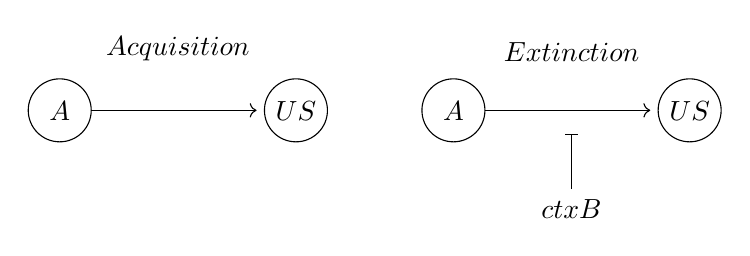
\begin{tikzpicture}
 	%A stage 2
 	\draw(7,2) circle(0.4);
 	\coordinate [label=$A$] (A) at (7, 1.75);
 	\draw[->](7.4,2) -- (9.5,2);
 	\draw(10,2) circle(0.4);
 	\draw[-|](8.5,1) -- (8.5,1.7);
 	\coordinate [label=$ctxB$] (B) at (8.5,0.5);
 	%A stage 1
 	\draw(2,2) circle(0.4);
 	\coordinate [label=$A$] (A) at (2, 1.75);
 	\draw[->](2.4,2) -- (4.5,2);
 	\draw(5,2) circle(0.4);
 	\coordinate [label=$US$] (X1) at (5, 1.75);
 	\coordinate [label=$Acquisition$] (S1) at (3.5,2.5);
 	\coordinate [label=$US$] (X1) at (10, 1.75);
 	\coordinate [label=$Extinction$] (S1) at (8.5,2.5);
 	\end{tikzpicture} } \\
 &
 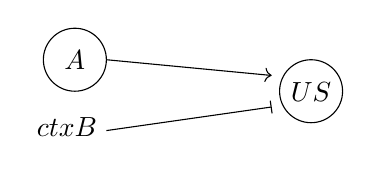
\begin{tikzpicture}
 %A stage 2
 \draw(7,2.4) circle(0.4);
 \coordinate [label=$A$] (A) at (7, 2.15);
 \coordinate [label=$US$] (X1) at (10, 1.75);
 \draw[->](7.4,2.4) -- (9.5,2.2);
 \coordinate [label=$ctxB$] (B) at (6.9,1.3);
 \draw[-|](7.4,1.5) -- (9.5,1.8);
 \draw(10,2) circle(0.4);
 \end{tikzpicture} \\
 \hline
 \end{tabular}
 \captionof{figure}{Illustration of first order and second order associative structures formed during acquisition and extinction (ctxB=context B). Arrow headed lines represented excitatory links, stopped lines represent inhibitory links. The \rwm suggests first order associations are formed during extinction (bottom-right) whereas an occasion setting model suggests second order associations are formed (top-right). See introductory text starting on pages \pageref{lab:extstr}-\pageref{lab:extstr1} for further details.}
 \label{fig:extinctionStructures}
 \end{table}
 
 \clearpage
 \begin{figure}[h]
  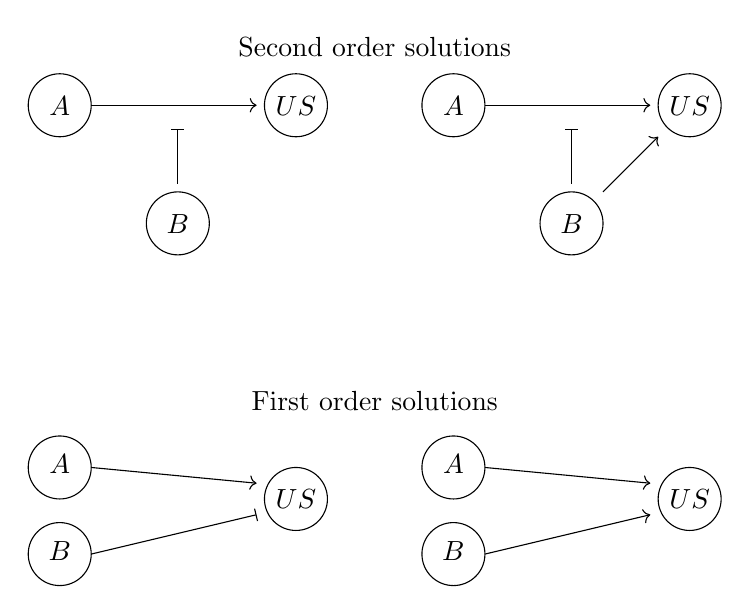
\begin{tikzpicture}
 %LHS top
    \draw(2,7) circle(0.4);
    \coordinate [label=$A$] (A) at (2, 6.75);
    \draw[->](2.4,7) -- (4.5,7);
    \draw(5,7) circle(0.4);
    \coordinate [label=$US$] (US) at (5, 6.75);
    \draw[-|](3.5,6) -- (3.5,6.7);
    \coordinate [label=$B$] (B) at (3.5,5.25);
    \draw(3.5,5.5) circle(0.4);
    \coordinate [label=Second order solutions] (S1) at (6,7.5);
 %LHS bottom
    \coordinate [label=First order solutions] (S1) at (6,3);
       \draw(2,2.4) circle(0.4);
       \coordinate [label=$A$] (A) at (2, 2.2);
       \coordinate [label=$US$] (US) at (5, 1.75);
       \draw[->](2.4,2.4) -- (4.5,2.2);
       \coordinate [label=$B$] (B) at (2,1.1);
       \draw(2,1.3) circle(0.4);
       \draw[-|](2.4,1.3) -- (4.5,1.8);
       \draw(5,2) circle(0.4);
       
 %RHS top
    \draw(7,7) circle(0.4);
    \coordinate [label=$A$] (A) at (7, 6.75);
    \draw[->](7.4,7) -- (9.5,7);
    \draw(10,7) circle(0.4);
    \coordinate [label=$US$] (US) at (10, 6.75);
    \draw[-|](8.5,6) -- (8.5,6.7);
    \coordinate [label=$B$] (B) at (8.5,5.25);
    \draw[->](8.9,5.9) -- (9.6,6.6);
    \draw(8.5,5.5) circle(0.4);
 %RHS bottom
       \draw(7,2.4) circle(0.4);
       \coordinate [label=$A$] (A) at (7, 2.2);
       \coordinate [label=$US$] (US) at (10, 1.75);
       \draw[->](7.4,2.4) -- (9.5,2.2);
       \coordinate [label=$B$] (B) at (7,1.1);
       \draw(7,1.3) circle(0.4);
       \draw[->](7.4,1.3) -- (9.5,1.8);
       \draw(10,2) circle(0.4);
    
  \end{tikzpicture}
  \caption{Status of first and second-order associative structures following training in a feature negative discrimination (left-hand side) and after reinforcement of the feature, B+ trials (right-hand side). See introductory text starting on page \pageref{lab:extstr1} for further details} \label{fig:reversalStructures}
  \end{figure}
 
\begin{comment}
\clearpage
\begin{figure}[ht]
	\begin{center}
		\begin{subfigure}[b]{0.45\textwidth}
\begin{knitrout}
\definecolor{shadecolor}{rgb}{0.969, 0.969, 0.969}\color{fgcolor}
\includegraphics[width=\maxwidth]{figure/TRACEAoE1-1} 

\end{knitrout}
			\caption{Experiment 1: Cue A} \label{fig:AtraceE1}
		\end{subfigure}
		\begin{subfigure}[b]{0.45\textwidth}
\begin{knitrout}
\definecolor{shadecolor}{rgb}{0.969, 0.969, 0.969}\color{fgcolor}
\includegraphics[width=\maxwidth]{figure/TRACEGoE1-1} 

\end{knitrout}
			\caption{cue D} \label{fig:GtraceE1}
		\end{subfigure} \\
		\begin{subfigure}[b]{0.45\textwidth}
\begin{knitrout}
\definecolor{shadecolor}{rgb}{0.969, 0.969, 0.969}\color{fgcolor}
\includegraphics[width=\maxwidth]{figure/TRACEAoE2-1} 

\end{knitrout}
			\caption{Experiment 2: Cue A} \label{fig:AtraceE2}
		\end{subfigure}
		\begin{subfigure}[b]{0.45\textwidth}
\begin{knitrout}
\definecolor{shadecolor}{rgb}{0.969, 0.969, 0.969}\color{fgcolor}
\includegraphics[width=\maxwidth]{figure/TRACEGoE2-1} 

\end{knitrout}
			\caption{cue D} \label{fig:GtraceE2}
		\end{subfigure} \\
\caption{Experiments 1 and 2 x-responses to cues A and G during acquisition, extinction, summation, and recovery test phases. Means $\pm$ 1 standard error.}
	\label{fig:aqexrt}
	\end{center}
\end{figure}
\end{comment}

\clearpage
\begin{figure}[ht]
\begin{center}
\begin{subfigure}[b]{0.45\textwidth}
\begin{knitrout}
\definecolor{shadecolor}{rgb}{0.969, 0.969, 0.969}\color{fgcolor}
\includegraphics[width=\maxwidth]{figure/TRACEA-1} 

\end{knitrout}
\caption{Cue A} \label{fig:Atrace}
\end{subfigure}
\begin{subfigure}[b]{0.45\textwidth}
\begin{knitrout}
\definecolor{shadecolor}{rgb}{0.969, 0.969, 0.969}\color{fgcolor}
\includegraphics[width=\maxwidth]{figure/TRACEG-1} 

\end{knitrout}
\caption{Cue D} \label{fig:Gtrace}
\end{subfigure} \\
\caption{Proportion of trials within blocks on which participants produced an x-response during Experiment 1. Left-hand side shows responses to cue A during acquisition (blocks 1-5), extinction (blocks 6-9), and recovery test (blocks 12, 13) phases. Right-hand side shows responses to cue D during acquisition (blocks 1-5) and summation test (blocks 10, 11) phases. Means $\pm$ 1 standard error.}
\label{fig:aqexrtc}
\end{center}
\end{figure}

\begin{comment}
\clearpage
\begin{figure}[ht]
\begin{center}
\begin{subfigure}[b]{0.45\textwidth}
\begin{knitrout}
\definecolor{shadecolor}{rgb}{0.969, 0.969, 0.969}\color{fgcolor}
\includegraphics[width=\maxwidth]{figure/FNE1-1} 

\end{knitrout}
\caption{Experiment 1: training} \label{fig:FNE1}
\end{subfigure}
\begin{subfigure}[b]{0.45\textwidth}
\begin{knitrout}
\definecolor{shadecolor}{rgb}{0.969, 0.969, 0.969}\color{fgcolor}
\includegraphics[width=\maxwidth]{figure/FNRE1-1} 

\end{knitrout}
\caption{reversal} \label{fig:FNRE1}
\end{subfigure} \\
\begin{subfigure}[b]{0.45\textwidth}
\begin{knitrout}
\definecolor{shadecolor}{rgb}{0.969, 0.969, 0.969}\color{fgcolor}
\includegraphics[width=\maxwidth]{figure/FNE2-1} 

\end{knitrout}
\caption{Experiment 2: training} \label{fig:FNE2}
\end{subfigure}
\begin{subfigure}[b]{0.45\textwidth}
\begin{knitrout}
\definecolor{shadecolor}{rgb}{0.969, 0.969, 0.969}\color{fgcolor}
\includegraphics[width=\maxwidth]{figure/FNRE2-1} 

\end{knitrout}
\caption{reversal} \label{fig:FNRE2}
\end{subfigure} \\
\caption{Experiments 1 and 2 outcome-likelihood ratings during feature negative training and feature reversal phases. Means $\pm$ 1 standard error.}
\label{fig:fnfnr}
\end{center}
\end{figure}
\end{comment}

\clearpage
\begin{figure}[ht]
\begin{center}
\begin{subfigure}[b]{0.45\textwidth}
\begin{knitrout}
\definecolor{shadecolor}{rgb}{0.969, 0.969, 0.969}\color{fgcolor}
\includegraphics[width=\maxwidth]{figure/FN-1} 

\end{knitrout}
\caption{Feature negative} \label{fig:FN}
\end{subfigure}
\begin{subfigure}[b]{0.45\textwidth}
\begin{knitrout}
\definecolor{shadecolor}{rgb}{0.969, 0.969, 0.969}\color{fgcolor}
\includegraphics[width=\maxwidth]{figure/FNR-1} 

\end{knitrout}
\caption{Feature reversal} \label{fig:FNR}
\end{subfigure} \\
\caption{Mean outcome ratings within block during Experiment 2. The left-hand side shows progression of the feature negative and feature positive discriminations that were learned during blocks 1-5. The right-hand side shows the progression during the reversal phase (blocks 6-9). Means $\pm$ 1 standard error.}
\label{fig:FNFNR}
\end{center}
\end{figure}

\begin{comment}
\clearpage
\begin{figure}[ht]
\begin{center}
\begin{subfigure}[b]{0.45\textwidth}
\begin{knitrout}
\definecolor{shadecolor}{rgb}{0.969, 0.969, 0.969}\color{fgcolor}
\includegraphics[width=\maxwidth]{figure/FNTE1-1} 

\end{knitrout}
\caption{Experiment 1} \label{fig:FNTE1}
\end{subfigure}
\begin{subfigure}[b]{0.45\textwidth}
\begin{knitrout}
\definecolor{shadecolor}{rgb}{0.969, 0.969, 0.969}\color{fgcolor}
\includegraphics[width=\maxwidth]{figure/FNTE2-1} 

\end{knitrout}
\caption{Experiment 2} \label{fig:FNTE2}
\end{subfigure} \\
\caption{Experiments 1 and 2 test for survival of feature negative discrimination following feature reversal. Means $\pm$ 1 standard error.}
\label{fig:fnt}
\end{center}
\end{figure}

\clearpage
\begin{figure}[ht]
\begin{center}
\begin{subfigure}[b]{0.45\textwidth}
\begin{knitrout}
\definecolor{shadecolor}{rgb}{0.969, 0.969, 0.969}\color{fgcolor}
\includegraphics[width=\maxwidth]{figure/InTestE1-1} 

\end{knitrout}
\caption{Experiment 1} \label{fig:INTE1}
\end{subfigure}
\begin{subfigure}[b]{0.45\textwidth}
\begin{knitrout}
\definecolor{shadecolor}{rgb}{0.969, 0.969, 0.969}\color{fgcolor}
\includegraphics[width=\maxwidth]{figure/InTestE2-1} 

\end{knitrout}
\caption{Experiment 2} \label{fig:INTE2}
\end{subfigure} \\
\begin{subfigure}[b]{0.9\textwidth}
\begin{knitrout}
\definecolor{shadecolor}{rgb}{0.969, 0.969, 0.969}\color{fgcolor}
\includegraphics[width=\maxwidth]{figure/InTestsAll-1} 

\end{knitrout}
\caption{Combined Experiments 1 and 2} \label{fig:INTALL}
\end{subfigure} \\
\caption{Top. Experiments 1 and 2 responses to AB compound in feature negative survival test for participants classified as non-inhibitors and inhibitors. Bottom. Data combined over Experiments 1 and 2. Means $\pm$ 1 standard error.}
\label{fig:inht}
\end{center}
\end{figure}
\end{comment}

\clearpage
\begin{figure}[ht]
\begin{center}
\begin{knitrout}
\definecolor{shadecolor}{rgb}{0.969, 0.969, 0.969}\color{fgcolor}
\includegraphics[width=\maxwidth]{figure/FNIT-1} 

\end{knitrout}
\caption{Mean outcome ratings within blocks during the Experiment 2 feature negative survival test for participants classified as inhibitors (Inh) or as non-inhibitors (NoInh) during the Experiment 1 summation test on cue $D$. Ratings averaged over blocks 10 and 11 for the reminder test on cue $I$, and over blocks 12 and 13 for the critical feature negative test on the $IJ$ cue compound. Means $\pm$ 1 standard error.} \label{fig:FNIT}
\end{center}
\end{figure}


\clearpage
\def\ms{15mm}
\def\plw{20mm}
\def\plh{20mm}
\begin{table}[t]
\begin{tabular}{lc}
\hline
\multirow{13}{*}{
	\begin{tikzpicture}[baseline=(current bounding box.north),
	ocircle/.style={circle,draw,minimum size=\ms},
	odcircle/.style={circle,draw,minimum size=\ms,double, double distance=2pt},
	shcircle/.style={circle,draw,minimum size=\ms,fill=black!20},
	orect/.style={rectangle,draw,minimum size=\ms},
	shrect/.style={rectangle,draw,minimum size=\ms,fill=black!20},
	plate/.style={rectangle, draw, rounded corners=3mm,minimum width=\plw, minimum height=\plh}]
	\node(p1) at (0,0) [plate,label=below:NoInh data]{};
	\node (xi) at (0,0) [shcircle] {\Large{$x_i$}};
	\node(p2) at (3,0) [plate,label=below:Inh data]{};
	\node (yj) at (3,0) [shcircle] {\Large{$y_j$}};
	\node (mu) at (-0.5,3)[ocircle]{\Large{$\mu$}}; 
	\node (sig) at (3.5,3)[ocircle]{\Large{$\sigma$}}; 
	\node (delta) at (1.5,4)[ocircle]{\Large{$\delta$}}; 
	\node (sigMu) at (-0.5,5.5)[odcircle]{\Large{$\sigma_\mu$}};
	\node (sigDelta) at (1.5,7)[odcircle]{\Large{$\sigma_\delta$}}; 
	\draw[-{>[scale=2.5,
		length=2,
		width=3]}](mu)--(xi);
	\draw[-{>[scale=2.5,
		length=2,
		width=3]}](mu)--(yj);
	\draw[-{>[scale=2.5,
		length=2,
		width=3]}](sig)--(xi);
	\draw[-{>[scale=2.5,
		length=2,
		width=3]}](sig)--(yj);
	\draw[-{>[scale=2.5,
		length=2,
		width=3]}](delta)--(yj);
	\draw[-{>[scale=2.5,
		length=2,
		width=3]}](sigMu)--(mu);
	\draw[-{>[scale=2.5,
		length=2,
		width=3]}](sigDelta)--(delta);
	\end{tikzpicture}} & \\   &  \\ & \\
& $\sigma_\delta \leftarrow 100 \times \sqrt{2} \times \sigma_{xy}$ \\
& $\sigma_\mu \leftarrow 100 \times \sigma_{xy}$ \\
& $\delta \sim$ Gaussian(0, $\sfrac{1}{\sigma_\delta^2}$)\\
& $\mu \sim$ Gaussian($\mu_{x}$,$\sfrac{1}{\sigma_\mu^2}$) \\
& $\sigma \sim$ Uniform($\sigma_{xy} \times \sfrac{1}{100}$, $\sigma_{xy} \times 100$) \\
& $x_i \sim$ Gaussian($\mu$, $\sfrac{1}{\sigma^2}$) \\
& $y_j \sim$ Gaussian($\mu+\delta$, $\sfrac{1}{\sigma^2}$) \\
& \\   & \\  & \\   & \\  
\hline \vspace{2pt}
\end{tabular}
\captionof{figure}{Graphical model for analysis to obtain posterior distributions (Figure \ref{fig:posteriors}) for the ratings of inhibitors and non-inhibitors in the feature negative survival test on $IJ$. $\sigma_{xy}$ is pooled standard deviation of observed data from both groups, $\mu_{x}$ is the mean of the data from the non-inhibitors group. The parameterisation of Gaussian distributions in JAGS is in terms of mean and precision where precision is $\sfrac{1}{\sigma^2}$}.
\label{tab:gm1}
\end{table}

\clearpage
\begin{figure}[ht]
\begin{center}
\begin{knitrout}
\definecolor{shadecolor}{rgb}{0.969, 0.969, 0.969}\color{fgcolor}
\includegraphics[width=\maxwidth]{figure/pltB2-1} 

\end{knitrout}
\caption{Jittered raw data and posterior distributions for the ratings given by the non-inhibitors and inhibitors in the feature negative survival test on $IJ$. The region of practical equivalence and the 95\% Bayesian credible interval are given around the means of the distributions for the non-inhibitors and the inhibitors, respectively. The posterior distributions generated according the model specification illustrated in Figure \ref{tab:gm1}.} 
\label{fig:posteriors}
\end{center}
\end{figure}

\begin{comment}
\begin{table}[t]
\begin{tabular}{lc}
\hline
\multirow{13}{*}{
	\begin{tikzpicture}[baseline=(current bounding box.north),
	ocircle/.style={circle,draw,minimum size=\ms},
	odcircle/.style={circle,draw,minimum size=\ms,double, double distance=2pt},
	shcircle/.style={circle,draw,minimum size=\ms,fill=black!20},
	orect/.style={rectangle,draw,minimum size=\ms},
	shrect/.style={rectangle,draw,minimum size=\ms,fill=black!20},
	plate/.style={rectangle, draw, rounded corners=3mm,minimum width=\plw, minimum height=\plh}]
	\node(p1) at (0,0) [plate,label=below:NoInh data]{};
	\node (xi) at (0,0) [shcircle] {\Large{$x_i$}};
	\node(p2) at (3,0) [plate,label=below:Inh data]{};
	\node (yj) at (3,0) [shcircle] {\Large{$y_j$}};
	\node (mu) at (-0.5,3)[ocircle]{\Large{$\mu$}}; 
	\node (sigma) at (3.5,3)[ocircle]{\Large{$\sigma$}}; 
	\node (alpha) at (1.5,4)[odcircle]{\Large{$\alpha$}}; 
	\node (delta) at (1.5,7)[ocircle]{\Large{$\delta$}}; 
	\draw[-{>[scale=2.5,
		length=2,
		width=3]}](mu)--(xi);
	\draw[-{>[scale=2.5,
		length=2,
		width=3]}](mu)--(yj);
	\draw[-{>[scale=2.5,
		length=2,
		width=3]}](sigma)--(xi);
	\draw[-{>[scale=2.5,
		length=2,
		width=3]}](sigma)--(yj);
	\draw[-{>[scale=2.5,
		length=2,
		width=3]}](alpha)--(yj);
	\draw[-{>[scale=2.5,
		length=2,
		width=3]}](sigma)--(alpha);
	\draw[-{>[scale=2.5,
		length=2,
		width=3]}](delta)--(alpha);
	\end{tikzpicture}} & \\   &  \\ & \\
& $\delta \sim$ Cauchy(0,1) \\
& $\mu \sim$ Cauchy(0,1) \\
& $\alpha \leftarrow \delta \sigma$ \\
& $\sigma \sim$ Cauchy(0,1)$[0,\infty]$ \\
& $x_i \sim$ Gaussian($\mu$, $\sfrac{1}{\sigma^2}$) \\
& $y_j \sim$ Gaussian($\mu+\alpha$, $\sfrac{1}{\sigma^2}$) \\
& \\   & \\  & \\   & \\  
\hline \vspace{2pt}
\end{tabular}
\captionof{figure}{Graphical model for Analysis 2. The parameterisation of Gaussian distributions in JAGS is in terms of mean and precision where precision is $\sfrac{1}{\sigma^2}$}
\label{tab:gm2}
\end{table}

\clearpage
\begin{figure}[ht]
\begin{center}
\begin{knitrout}
\definecolor{shadecolor}{rgb}{0.969, 0.969, 0.969}\color{fgcolor}
\includegraphics[width=\maxwidth]{figure/pltB1-1} 

\end{knitrout}
\caption{Prior and posterior distributions for the effect size ($\delta$) on the difference between the group means for non-inhibitors and inhibitors in the AB compound test. The relative values of the distributions is given at $\delta =0$ and the 95\% Bayesian credible interval is given around the mean of the posterior distribution.} 
\label{fig:effectsizes}
\end{center}
\end{figure}
\end{comment}

\end{document}
